\documentclass[11pt]{article}
\usepackage[english]{babel}
\usepackage[utf8]{inputenc}
\usepackage[margin=0.5in]{geometry}
\usepackage{amsmath}
\usepackage{amsthm}
\usepackage{amsfonts}
\usepackage{amssymb}
\usepackage[usenames,dvipsnames]{xcolor}
\usepackage{graphicx}
\usepackage[siunitx]{circuitikz}
\usepackage{tikz}
\usepackage[colorinlistoftodos, color=orange!50]{todonotes}
\usepackage{hyperref}
\usepackage[numbers, square]{natbib}
\usepackage{fancybox}
\usepackage{epsfig}
\usepackage{soul}
\usepackage[framemethod=tikz]{mdframed}
\usetikzlibrary{positioning, automata, backgrounds}
\usepackage[shortlabels]{enumitem}
\usepackage[version=4]{mhchem}
\usepackage{multicol}
\usepackage{forest}
\usepackage{mathtools}
\usepackage{comment}
\usepackage{enumitem}
\usepackage[utf8]{inputenc}
\usepackage[linesnumbered,ruled,vlined]{algorithm2e}
\usepackage{listings}
\usepackage{color}
\usepackage[numbers]{natbib}
\usepackage{subfiles}
\usepackage{tkz-berge}


\newcommand{\interval}[4]{\draw (#2, #1) -- (#3, #1); % Usage: \interval{height}{start}{end}{label}
\draw (#2, #1-0.11) -- (#2, #1+0.11); % draw left whisker
\draw (#3, #1-0.11) -- (#3, #1+0.11); % draw right whisker
\node[] at (#2-0.25, #1) {#4};
}

\newtheorem{prop}{Proposition}[section]
\newtheorem{thm}{Theorem}[section]
\newtheorem{lemma}{Lemma}[section]
\newtheorem{cor}{Corollary}[prop]

\theoremstyle{definition}
\newtheorem{definition}{Definition}

\theoremstyle{definition}
\newtheorem{required}{Problem}

\theoremstyle{definition}
\newtheorem{ex}{Example}


\setlength{\marginparwidth}{3.4cm}
%#########################################################

%To use symbols for footnotes
\renewcommand*{\thefootnote}{\fnsymbol{footnote}}
%To change footnotes back to numbers uncomment the following line
%\renewcommand*{\thefootnote}{\arabic{footnote}}

% Enable this command to adjust line spacing for inline math equations.
% \everymath{\displaystyle}

% _______ _____ _______ _      ______ 
%|__   __|_   _|__   __| |    |  ____|
%   | |    | |    | |  | |    | |__   
%   | |    | |    | |  | |    |  __|  
%   | |   _| |_   | |  | |____| |____ 
%   |_|  |_____|  |_|  |______|______|
%%%%%%%%%%%%%%%%%%%%%%%%%%%%%%%%%%%%%%%

\title{
\normalfont \normalsize 
\textsc{CSCI 3104 Spring 2023 \\ 
Instructors: Ryan Layer and Chandra Kanth Nagesh} \\
[10pt] 
\rule{\linewidth}{0.5pt} \\[6pt] 
\huge Homework 7 \\
\rule{\linewidth}{2pt}  \\[10pt]
}
%\author{}
\date{}

\begin{document}

\definecolor {processblue}{cmyk}{0.96,0,0,0}
\definecolor{processred}{rgb}{200, 0, 0}
\definecolor{processgreen}{rgb}{0, 255, 0}
\DeclareGraphicsExtensions{.png}
\DeclareGraphicsExtensions{.gif}
\DeclareGraphicsExtensions{.jpg}

\maketitle


%%%%%%%%%%%%%%%%%%%%%%%%%
%%%%%%%%%%%%%%%%%%%%%%%%%%
%%%%%%%%%%FILL IN YOUR NAME%%%%%%%
%%%%%%%%%%AND STUDENT ID%%%%%%%%
%%%%%%%%%%%%%%%%%%%%%%%%%%
\noindent
Due Date \dotfill February 16, 2023 \\
Name \dotfill \textbf{Blake Raphael} \\
Student ID \dotfill \textbf{109752312} \\
Collaborators \dotfill \textbf{Alex Barry and Brody Cyphers}

\tableofcontents

\section{Instructions}
 \begin{itemize}
	\item The solutions \textbf{should be typed}, using proper mathematical notation. We cannot accept hand-written solutions. \href{http://ece.uprm.edu/~caceros/latex/introduction.pdf}{Here's a short intro to \LaTeX.}
	\item You should submit your work through the \textbf{class Gradescope page} only (linked from Canvas). Please submit one PDF file, compiled using this \LaTeX \ template.
	\item You may not need a full page for your solutions; pagebreaks are there to help Gradescope automatically find where each problem is. Even if you do not attempt every problem, please submit this document with no fewer pages than the blank template (or Gradescope has issues with it).

	\item You are welcome and encouraged to collaborate with your classmates, as well as consult outside resources. You must \textbf{cite your sources in this document.} \textbf{Copying from any source is an Honor Code violation. Furthermore, all submissions must be in your own words and reflect your understanding of the material.} If there is any confusion about this policy, it is your responsibility to clarify before the due date. 

	\item Posting to \textbf{any} service including, but not limited to Chegg, Reddit, StackExchange, etc., for help on an assignment is a violation of the Honor Code.

	\item You \textbf{must} virtually sign the Honor Code (see Section \ref{HonorCode}). Failure to do so will result in your assignment not being graded.
\end{itemize}


\section{Honor Code (Make Sure to Virtually Sign)} \label{HonorCode}

%\begin{required}
\begin{itemize}
\item My submission is in my own words and reflects my understanding of the material.
\item Any collaborations and external sources have been clearly cited in this document.
\item I have not posted to external services including, but not limited to Chegg, Reddit, StackExchange, etc.
\item I have neither copied nor provided others solutions they can copy.
\end{itemize}

%\noindent In the specified region below, clearly indicate that you have upheld the Honor Code. Then type your name. 
%\end{required}

\begin{proof}[Agreed (I agree to the above, Blake Raphael).]
%% Typing "I agree to the above," followed by your name is sufficient.
\end{proof}

\newpage
\section{Standard 7: Kruskal's MST Algorithm}
\setcounter{subsection}{1}
\subsection{Problem \ref{MST_Kruskal} (2 points)}
\begin{required} \label{MST_Kruskal}
Consider the weighted graph $G(V, E, w)$ below. Clearly list the order in which Kruskal's algorithm adds edges to a minimum-weight spanning tree for $G$. Additionally, clearly articulate the steps that Kruskal's algorithm takes as it selects the first \textbf{three} edges.


\begin{center}
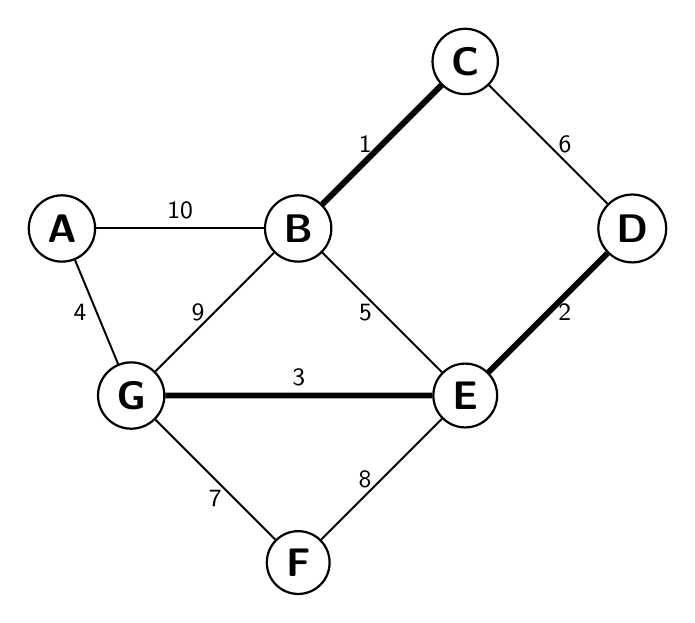
\begin{tikzpicture}[scale=0.4, auto, node distance=3cm, every loop/.style={},
thick,main node/.style={circle,draw,font=\sffamily\Large\bfseries}]

\node[main node] (A) {A};
\node[main node] (B) [right of=A] {B};
\node[main node] (C) [above right of=B] {C};
\node[main node] (D) [below right of=C] {D};
\node[main node] (E) [below left of=D] {E};
\node[main node] (F) [below left of=E] {F};
\node[main node] (G) [above left of=F] {G};

\path[line width=0.25mm, every node/.style={font=\sffamily\small}]
(B) edge node [left]  {1} (C)
(B) edge node [left]  {5}  (E)
(C) edge node [right] {6}  (D)
(D) edge node [right] {2} (E)
(F) edge node [below] {7} (G)
(G) edge node [above] {3}  (E)
(A) edge node [left] {4} (G)
(A) edge node [above] {10} (B)
(E) edge node [left] {8} (F)
(B) edge node [left] {9} (G)
;

\draw[line width=0.75mm] (B) -- (C);
\draw[line width=0.75mm] (E) -- (D);
\draw[line width=0.75mm] (G) -- (E);
\end{tikzpicture}
\end{center}
\end{required}

\begin{proof}
Kruskal's algorithm adds the edges in the following order:\\
1: $\{B, C\}$\\
2: $\{D, E\}$\\
3: $\{G, E\}$\\
4: $\{A, G\}$\\
5: $\{B, E\}$\\
6: $\{F, E\}$\\

First we add all the edges to the priority queue ordered in ascending order based on edge weights. Next, we check if the edge creates a cycle or there is already a path connecting those vertices. If not, we add the edge and pop it from the queue. For the first 3 edges, we check if $\{B, C\}$ creates a cycle or there is a path between the two. Since it does neither, we add that edge and pop $\{B, C\}$ from the queue. Next we check if $\{D, E\}$ creates a cycle or there is a path between the two. Since it does neither, we add that edge and pop $\{D, E\}$ from the queue. Next we check if $\{G, E\}$ creates a cycle or there is a path between the two. Since it does neither, we add that edge and pop $\{G, E\}$ from the queue.
\end{proof}


\newpage
\section{Standard 7: Prim's MST Algorithm}
\subsection{Problem \ref{MST_Priml} (2 points)}
\begin{required} \label{MST_Priml}
Consider the weighted graph $G(V, E, w)$ below. Clearly list the order in which Kruskal's algorithm adds edges to a minimum-weight spanning tree for $G$. Additionally, clearly articulate the steps that Kruskal's algorithm takes as it selects the first \textbf{three} edges.
Consider the weighted graph $G(V, E, w)$ below. Clearly list the order in which Prim's algorithm, \textbf{using the source vertex} $A$, adds edges to a minimum-weight spanning tree for $G$. Additionally, clearly articulate the steps that Prim's algorithm takes as it selects the first \textbf{three} edges.

\begin{center}
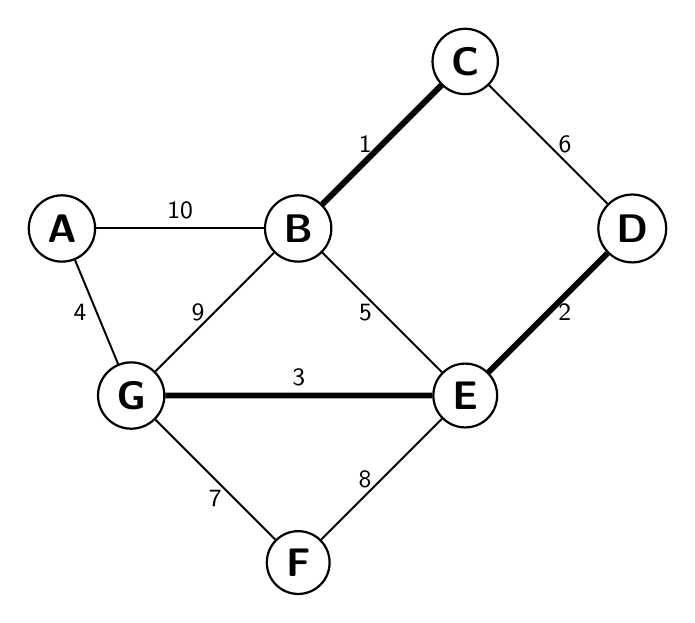
\begin{tikzpicture}[scale=0.4, auto, node distance=3cm, every loop/.style={},
  thick,main node/.style={circle,draw,font=\sffamily\Large\bfseries}]

\node[main node] (A) {A};
\node[main node] (B) [right of=A] {B};
\node[main node] (C) [above right of=B] {C};
\node[main node] (D) [below right of=C] {D};
\node[main node] (E) [below left of=D] {E};
\node[main node] (F) [below left of=E] {F};
\node[main node] (G) [above left of=F] {G};

\path[line width=0.25mm, every node/.style={font=\sffamily\small}]
(B) edge node [left]  {1} (C)
(B) edge node [left]  {5}  (E)
(C) edge node [right] {6}  (D)
(D) edge node [right] {2} (E)
(F) edge node [below] {7} (G)
(G) edge node [above] {3}  (E)
(A) edge node [left] {4} (G)
(A) edge node [above] {10} (B)
(E) edge node [left] {8} (F)
(B) edge node [left] {9} (G)
;

\draw[line width=0.75mm] (B) -- (C);
\draw[line width=0.75mm] (E) -- (D);
\draw[line width=0.75mm] (G) -- (E);
\end{tikzpicture}
\end{center}
\end{required}

\begin{proof}
Prim's algorithm adds the edges in the following order:\\
1: $\{A, G\}$\\
2: $\{G, E\}$\\
3: $\{E, D\}$\\
4: $\{E, B\}$\\
5: $\{B, C\}$\\
6: $\{G, F\}$\\

First we add all the edges to the priority queue ordered in ascending order based on edge weights starting from our source node. Next, we check if the edge creates a cycle or there is already a path connecting those vertices. We add edges to the priority queue if they are child nodes from the source node or children nodes of the source node. If not, we add the edge and pop it from the queue. For the first 3 edges, we check if $\{A, G\}$ creates a cycle or there is a path between the two. Since it does neither, we add that edge and pop $\{A, G\}$ from the queue. Next we check if $\{G, E\}$ creates a cycle or there is a path between the two. Since it does neither, we add that edge and pop $\{G, E\}$ from the queue. Next we check if $\{E, D\}$ creates a cycle or there is a path between the two. Since it does neither, we add that edge and pop $\{E, D\}$ from the queue.
\end{proof}

\end{document} % NOTHING AFTER THIS LINE IS PART OF THE DOCUMENT
